\chapter{\ChapterTitleResults}
\label{sec:wyniki-projektu}

\section{Weryfikacja realizacji wstępnych założeń}

W~pierwszym etapie planowania projektu utworzony został ogólny
plan, który opisywał oddzielne systemy i~elementy
zleconej aplikacji (Rys. \ref{fig:figma_strategicplan}).
Uwzględnia on nie tylko wymagania zdefiniowane w~rozdziale drugim
\nameref{sec:zakres-funkcjonalnosci}, ale także potrzebne do ich
realizacji wymagania techniczne.

\begin{figure}[h!]
    \centering
    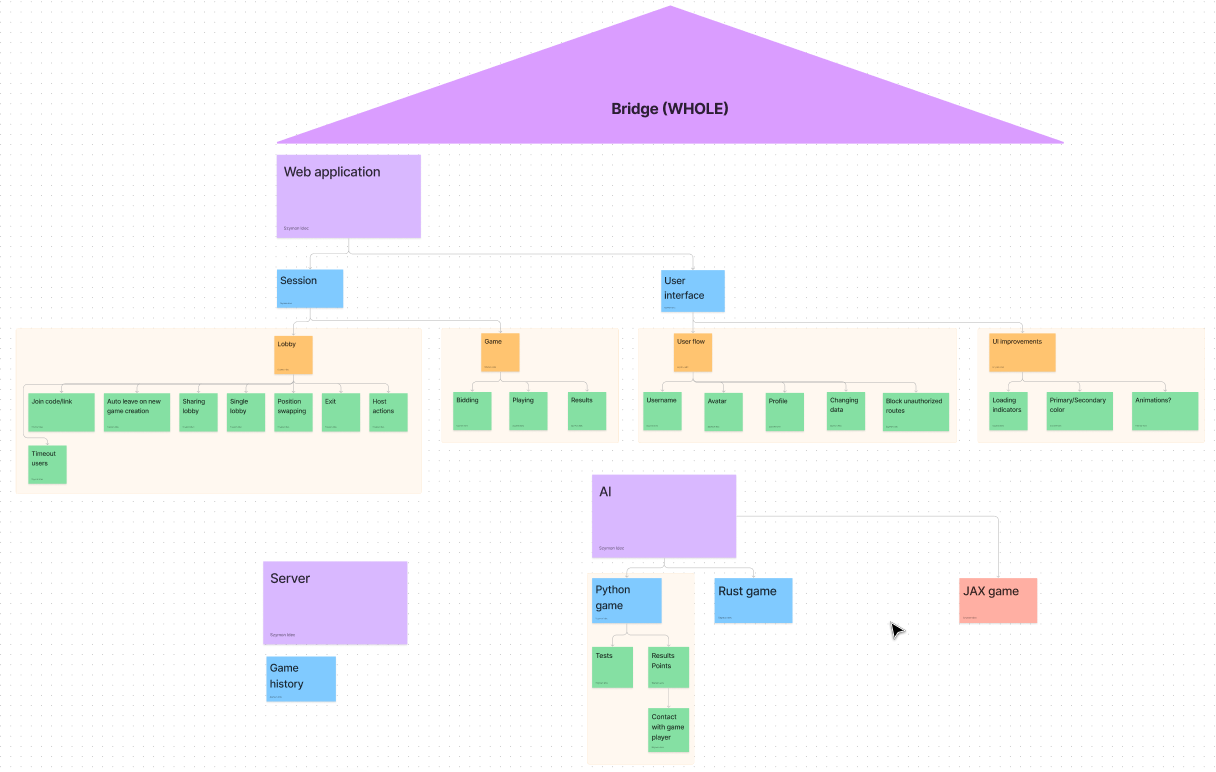
\includegraphics[width=0.9\textwidth]{img/schematy/milestones.png}
    \caption{Szczegółowy podział milestone'ów na zadania}
    \label{fig:figma_strategicplan}
\end{figure}

Opierając się na powyższym planie, można stwierdzić, że udało się
zrealizować wszystkie wymagania sprecyzowane przez klienta.
Jedynym elementem, który został zrealizowany alternatywnie,
zgodnie z~założeniami zagrożeń implementacji
(\nameref{sec:analiza_zagrozen}), był wirtualny asystent. Szczegóły
dotyczące tej części projektu zostały opisane w~sekcji dotyczącej
asystenta \nameref{subsubsec:mocai}.

\section{Przegląd zrealizowanych funkcjonalności}

\subsection{Interfejs aplikacji}

\subsubsection{Tworzenie i dołączenie do gry}
\subsubsection{Lobby}
\subsubsection{Host}
\subsubsection{Użytkownik}


\subsection{Gra w brydża}

\subsubsection{Licytacja}
\subsubsection{Rozgrywka}


\subsection{Wirtualny asystent}
%%% przeprowadzone testy aplikacji na wybranej grupie osób (do wywalenia?)

\subsubsection{Moc AI}
\label{subsubsec:mocai}
%%% testy/badania czy AI wygrywa

\subsubsection{Możliwości rozwoju modelu}
%%% czy da sie rozszerzac o kolejne elementy gry brydza
%%% mozna sie odwolac do dalszych perspektyw (na ten moment w PR)

\subsection{Ułatwienia dostępności}

Oprócz omówionych kluczowych funkcjonalności, w~ramach rozwoju
aplikacji wprowadzono także dodatkowe elementy, których
potrzebę przedstawiono w~podrozdziale dotyczącym wymagań
niefunkcjonalnych. Głównych ich celem było zapewnienie
wygody i~prostego korzystania z~aplikacji, nawet podczas
pierwszego użytkowania. Poniżej przedstawione rozwiązania powstały
z~inicjatywy zespołu. Zostały one zaakceptowane przez klienta,
realizując wymagania dostępności i~użyteczności.

\subsubsection{Intuicyjność interfejsu}

Aby aplikacja była intuicyjna dla każdego użytkownika,
zastosowano ikony wprost kojarzące się z~wykonywaną
przez nie akcją. Zastosowano wyróżniające się kolory wśród palety
aplikacji w~celu podkreślenia danych czynności wykonywanych
przez użytkownika (Rys. \ref{fig:host_actions_ui}). Kontrastowe barwy mają zwrócić uwagę na
skutki danej akcji. Przykładowo jaskrawy czerwony kolor
kojarzący się przemocą lub impulsywnością wraz z~ikoną
przedstawiającą "$\times$"\xspace odpowiada za wyrzucenie gracza
z~sesji. Zastosowanie wspomnianych technik przestrzega
użytkownika przed przedwczesnym kliknięciem, ale także kojarzą
się one z~negatywną czynnością.

\begin{figure}[h!]
  \centering
  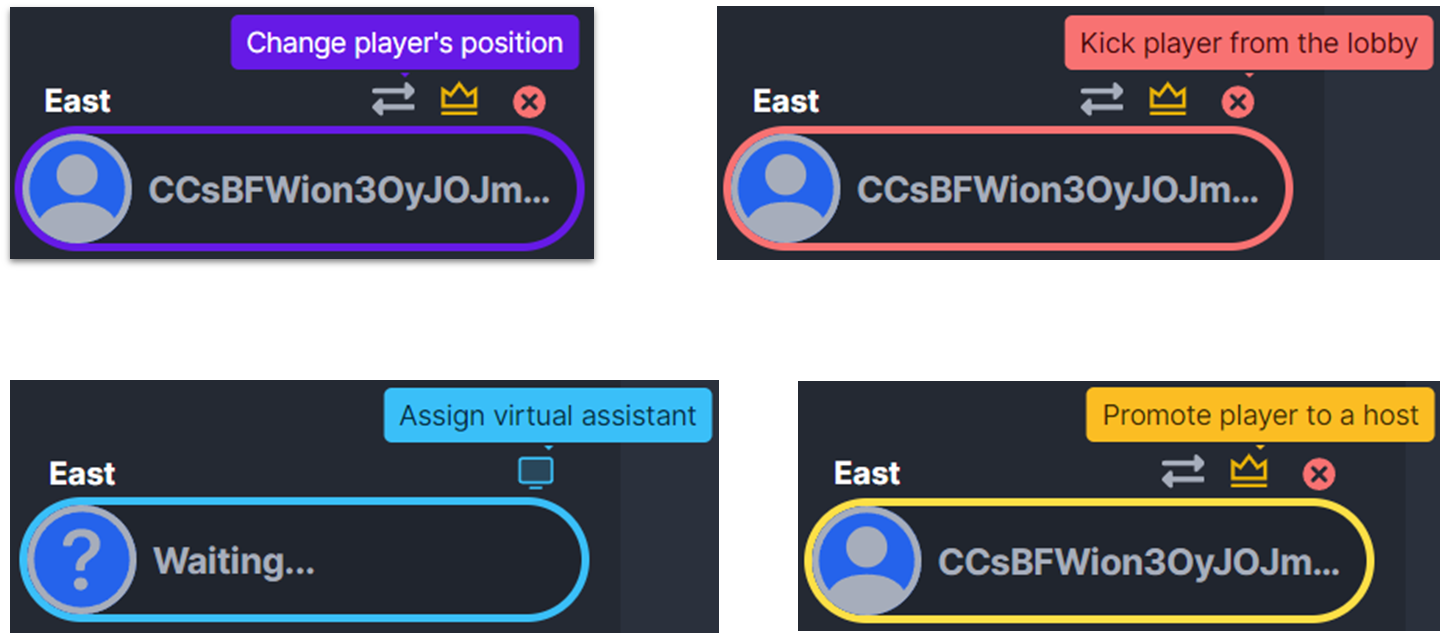
\includegraphics[width=\textwidth]{img/widoki/host_actions.png}
  \caption{Akcje hosta lobby}
  \label{fig:host_actions_ui}
\end{figure}

\FloatBarrier

\subsubsection{Responsywny układ aplikacji}

Zgodnie z~wymogiem dostępności interfejsy aplikacji powinny
być funkcjonalne również na urządzeniach o~niewielkich
rozmiarach ekranu. Wszystkie strony zostały zaprojektowane
tak, aby umożliwić wygodne korzystanie zarówno na urządzeniach
stacjonarnych, jak i~mobilnych (Rys. \ref{fig:responsive_ui}). Aplikacja dynamicznie
dostosowuje się w~zależności od aktualnego rozmiaru okna
przeglądarki.

Minimalna przewidziana
szerokość ekranu wynosi 280 pikseli, dzięki czemu wspierane
są także starsze urządzenia o~niewielkiej rozdzielczości
ekranu.

\begin{figure}[h!]
  \centering
  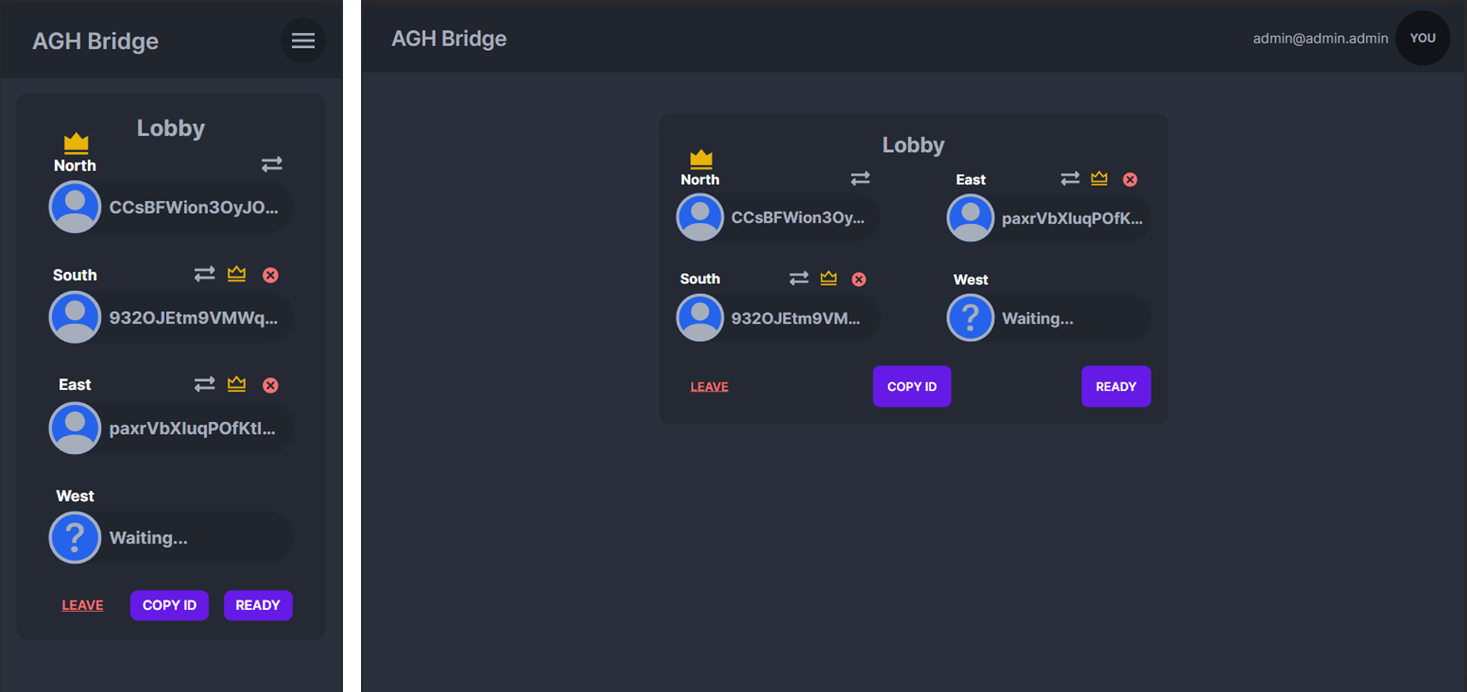
\includegraphics[width=\textwidth]{img/widoki/desktop_mobile.png}
  \caption{Tryb mobilny i desktopowy aplikacji}
  \label{fig:responsive_ui}
\end{figure}

\FloatBarrier

\subsubsection{Motywy jasny i ciemny}

Wygląd aplikacji został zrealizowany w~dwóch trybach --
jasnym i~ciemnym (Rys. \ref{fig:themes_ui}). Użyto w~tym celu dostępnych w~bibliotece
palet kolorów, ale także zdefiniowano własne, aby zachować
motyw kolorystyczny aplikacji. W~zależności od aktualnie
wybranego motywu kolory zmieniały swój odcień.

% \begin{figure}[h!]
%   \centering
%   \includegraphics[width=\textwidth, draft=true]{example-image}
%   \caption{Motywy jasny i ciemny aplikacji}
%   \label{fig:themes_ui}
% \end{figure}

% \FloatBarrier

\begin{figure}[h!]
  \centering
  \begin{minipage}[b]{0.45\textwidth}
    \centering
    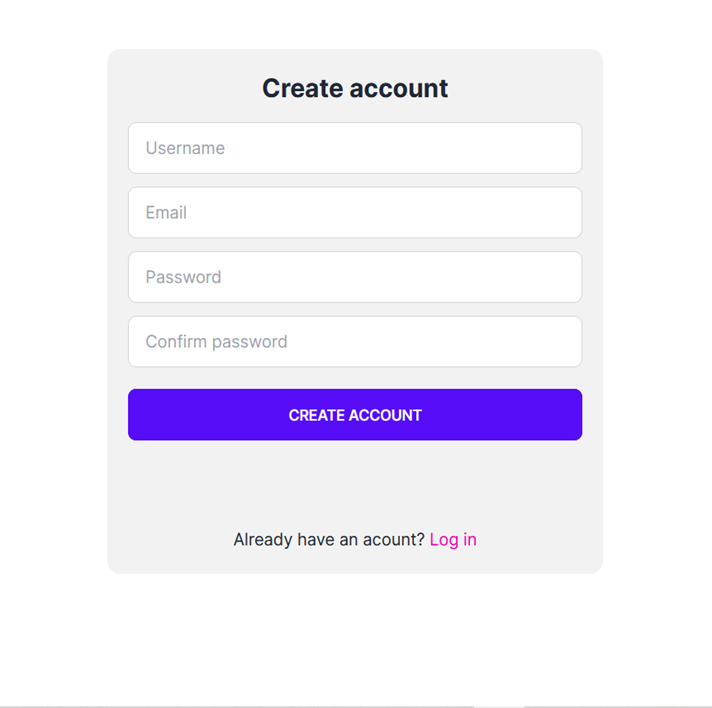
\includegraphics[width=\textwidth]{img/widoki/light.png}
  \end{minipage}%
  \hspace*{0.5cm}
  \begin{minipage}[b]{0.45\textwidth}
    \centering
    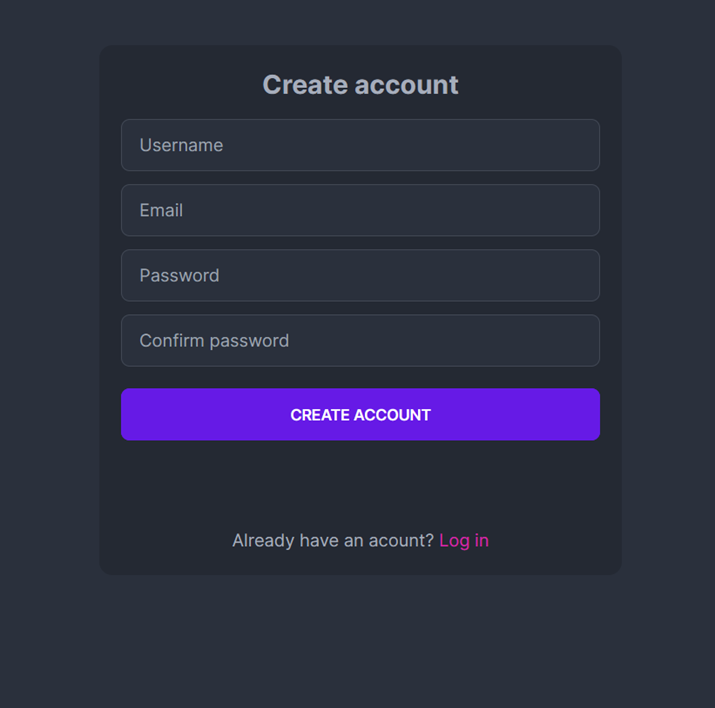
\includegraphics[width=\textwidth]{img/widoki/dark.png}
  \end{minipage}
  \caption{Motywy jasny i ciemny aplikacji}
  \label{fig:themes_ui}
\end{figure}

\FloatBarrier

\section{Dalsze perspektywy rozwoju projektu}

\section{Podsumowanie}


